% automatically generated document using lt2circuiTikz
\documentclass[tikz,margin={2pt 2pt 2pt 2pt}]{standalone}
\usepackage[compatibility,siunitx,  americanvoltages, americancurrents, europeanresistors, europeaninductors, americanports,%
  straightlabels, fetbodydiode, straightvoltages]{circuitikz}
\usepackage{tikz,amsmath, amssymb,bm,color,pgfkeys,siunitx,ifthen,ulem}
\usepackage{pgfplots}
\pgfplotsset{compat=1.14}
\usetikzlibrary{shapes,arrows}
%\usepackage{agaramondc}					% Adobe Garamond, custom shape
%\renewcommand{\shapedefault}{rtl} % rtl: roman tabular lining

\makeatletter

%% bandstop filter (adapted from highpass)
\pgfcircdeclarebipole{}{\ctikzvalof{bipoles/highpass/width}}{*bandstop}{\ctikzvalof{bipoles/highpass/width}}{\ctikzvalof{bipoles/highpass/width}}{
	\pgf@circ@res@step = \ctikzvalof{bipoles/highpass/width}\pgf@circ@Rlen
	\divide \pgf@circ@res@step by 2
	
	\pgfpathmoveto{\pgfpoint{\pgf@circ@res@left}{\pgf@circ@res@zero}}
	\pgf@circ@res@other = \pgf@circ@res@left
	\advance\pgf@circ@res@other by \pgf@circ@res@step 
	
	\ifpgf@circuit@dashed
	\pgfsetdash{{0.1cm}{0.1cm}}{0cm} 
	\fi	
	
	% draw outer box
	\pgfsetlinewidth{\pgfkeysvalueof{/tikz/circuitikz/bipoles/thickness}\pgfstartlinewidth}
	\pgfpathrectanglecorners{\pgfpoint{\pgf@circ@res@left}{\pgf@circ@res@up}}{\pgfpoint{\pgf@circ@res@right}{\pgf@circ@res@down}}
	\pgfusepath{draw}
	
	\ifpgf@circuit@inputarrow
	{
		\advance \pgf@circ@res@left by -.5\pgfkeysvalueof{/tikz/circuitikz/bipoles/thickness}\pgfstartlinewidth
		\pgftransformshift{\pgfpoint{\pgf@circ@res@left}{0pt}}
		\pgfnode{inputarrow}{tip}{}{pgf@inputarrow}{\pgfusepath{fill}}
	}
	\fi
	
	% rotate inner symbol
	\def\pgfcircmathresult{\expandafter\pgf@circ@stripdecimals\pgf@circ@direction\pgf@nil}
	\ifnum \pgfcircmathresult > 45 \ifnum \pgfcircmathresult < 135
	\pgftransformrotate{270}
	\fi\fi
	\ifnum \pgfcircmathresult > 134 \ifnum \pgfcircmathresult < 225  % 134 degree, because >= 135 is not possible
	\pgftransformrotate{180}
	\fi\fi
	\ifnum \pgfcircmathresult > 224 \ifnum \pgfcircmathresult < 315
	\pgftransformrotate{90}
	\fi\fi
	
	% draw inner symbol
	\pgfsetdash{}{0pt}	% always draw solid line for inner symbol
	\pgfsetarrows{-} %never draw arrows
	\pgfsetlinewidth{\pgfstartlinewidth}
	\pgfpathmoveto{\pgfpoint{-0.5\pgf@circ@res@step}{0.5\pgf@circ@res@step}}
	\pgfpathsine{\pgfpoint{.25\pgf@circ@res@step}{.25\pgf@circ@res@step}}
	\pgfpathcosine{\pgfpoint{.25\pgf@circ@res@step}{-.25\pgf@circ@res@step}}
	\pgfpathsine{\pgfpoint{.25\pgf@circ@res@step}{-.25\pgf@circ@res@step}}
	\pgfpathcosine{\pgfpoint{.25\pgf@circ@res@step}{.25\pgf@circ@res@step}}
	\pgfusepath{draw}
	
	\pgfpathmoveto{\pgfpoint{-0.5\pgf@circ@res@step}{0}}
	\pgfpathsine{\pgfpoint{.25\pgf@circ@res@step}{.25\pgf@circ@res@step}}
	\pgfpathcosine{\pgfpoint{.25\pgf@circ@res@step}{-.25\pgf@circ@res@step}}
	\pgfpathsine{\pgfpoint{.25\pgf@circ@res@step}{-.25\pgf@circ@res@step}}
	\pgfpathcosine{\pgfpoint{.25\pgf@circ@res@step}{.25\pgf@circ@res@step}}
	\pgfusepath{draw}
	\pgfpathmoveto{\pgfpoint{-0.15\pgf@circ@res@step}{-0.15\pgf@circ@res@step}}
	\pgfpathlineto{\pgfpoint{0.15\pgf@circ@res@step}{0.15\pgf@circ@res@step}}
	\pgfusepath{draw}
	
	\pgfpathmoveto{\pgfpoint{-0.5\pgf@circ@res@step}{-0.5\pgf@circ@res@step}}
	\pgfpathsine{\pgfpoint{.25\pgf@circ@res@step}{.25\pgf@circ@res@step}}
	\pgfpathcosine{\pgfpoint{.25\pgf@circ@res@step}{-.25\pgf@circ@res@step}}
	\pgfpathsine{\pgfpoint{.25\pgf@circ@res@step}{-.25\pgf@circ@res@step}}
	\pgfpathcosine{\pgfpoint{.25\pgf@circ@res@step}{.25\pgf@circ@res@step}}
	\pgfusepath{draw}
	%	\pgfpathmoveto{\pgfpoint{-0.15\pgf@circ@res@step}{-0.65\pgf@circ@res@step}}
	%	\pgfpathlineto{\pgfpoint{0.15\pgf@circ@res@step}{-0.35\pgf@circ@res@step}}
	%	\pgfusepath{draw}
}

\tikzset{
	*bandstop/.style={\circuitikzbasekey, /tikz/to path=\pgf@circ@*bandstop@path},
}
\def\pgf@circ@*bandstop@path#1{\pgf@circ@bipole@path{*bandstop}{#1}}




\makeatother

\usetikzlibrary{backgrounds,calc,positioning}

\usetikzlibrary{circuits.ee.IEC}
\usetikzlibrary{arrows}


% sym32a style

\ctikzset{tripoles/mos style/arrows}
\ctikzset{
	/tikz/circuitikz/quadpoles/coupler/width=1,%1.3
	/tikz/circuitikz/quadpoles/coupler/height=0.952,%1.3
	/tikz/circuitikz/quadpoles/coupler2/width=1,%1.3
	/tikz/circuitikz/quadpoles/coupler2/height=0.952,%1.3
	/tikz/circuitikz/quadpoles/transformer/width=1.425,%1.5
	/tikz/circuitikz/quadpoles/transformer/height=1.425,%1.5
	/tikz/circuitikz/quadpoles/transformer core/width=1.425,%1.5
	/tikz/circuitikz/quadpoles/transformer core/height=1.425,%1.5
	/tikz/circuitikz/quadpoles/gyrator/width=1.425,%1.5
	/tikz/circuitikz/quadpoles/gyrator/height=1.425,%1.5
	%/tikz/circuitikz/monopoles/tlinestub/width=0.1875,%0.25 no effect!
	/tikz/circuitikz/tripoles/american and port/height=0.95,%.8
	/tikz/circuitikz/tripoles/american nand port/height=0.95,%.8
	/tikz/circuitikz/tripoles/american or port/height=0.95,%.8
	/tikz/circuitikz/tripoles/american nor port/height=0.95,%.8
	/tikz/circuitikz/tripoles/american xor port/height=0.95,%.8
	/tikz/circuitikz/tripoles/american xnor port/height=0.95,%.8
	/tikz/circuitikz/bipoles/tline/height=0.4,%0.3
%	/tikz/circuitikz/bipoles/tline/width=1.2,%0.8
	/tikz/circuitikz/bipoles/diode/height=0.375,%
	/tikz/circuitikz/bipoles/diode/width=0.375,%
	/tikz/circuitikz/bipoles/varcap/height=0.375,%
	/tikz/circuitikz/bipoles/varcap/width=0.375,%
	/tikz/circuitikz/tripoles/triac/height=1.05,%
	/tikz/circuitikz/tripoles/triac/width=0.952,%
	/tikz/circuitikz/tripoles/thyristor/height=1.05,%
	/tikz/circuitikz/tripoles/thyristor/width=0.952,%
	/tikz/circuitikz/tripoles/op amp/height=0.952,%
	/tikz/circuitikz/tripoles/op amp/width=1.2,%
	/tikz/circuitikz/tripoles/op amp/font=\footnotesize,
	/tikz/circuitikz/tripoles/gm amp/height=0.952,% 1.7
	/tikz/circuitikz/tripoles/gm amp/width=1.2,% 1.4
	%	/tikz/circuitikz/tripoles/gm amp/font=\footnotesize,
	/tikz/circuitikz/tripoles/plain amp/height=0.952,% 1.7
	/tikz/circuitikz/tripoles/plain amp/width=1.2,% 1.4
	/tikz/circuitikz/bipoles/resistor/voltage/straight label distance/.initial=.8,
	/tikz/circuitikz/bipoles/generic/voltage/straight label distance/.initial=.8,
	/tikz/circuitikz/bipoles/inductor/voltage/straight label distance/.initial=.8,
	/tikz/circuitikz/bipoles/fullgeneric/voltage/straight label distance/.initial=.8,
	/tikz/circuitikz/bipoles/capacitor/voltage/straight label distance/.initial=1.0,
	/tikz/circuitikz/bipoles/thickness=1.6,
}
\ctikzset{v/.append style={/tikz/european voltages}}

\definecolor{netlabelcolor}{rgb}{0, 0, 0.25}
\definecolor{lttotitextcolor}{rgb}{0, 0.4, 0.25}
\definecolor{lttotidrawcolor}{rgb}{0.6, 0.6, 0.6}
\definecolor{netcolor}{rgb}{0, 0, 0.5}

\pgfkeys{/lt2ti/netlabel/font/.initial= \small}
\pgfkeys{/lt2ti/text/font/.initial= \small}

\pgfkeys{/lt2ti/Net/.style= {netcolor}}
\tikzstyle{dashdotdotted}=[dash pattern=on 3pt off 2pt on \the\pgflinewidth off 2pt on \the\pgflinewidth off 2pt]

\pgfkeys{/lt2ti/VArrow/.style= {->,>=latex}}
\pgfkeys{/lt2ti/SArrow/.style= {->,>=angle 90}}

\begin{document}%
	%\centering%
		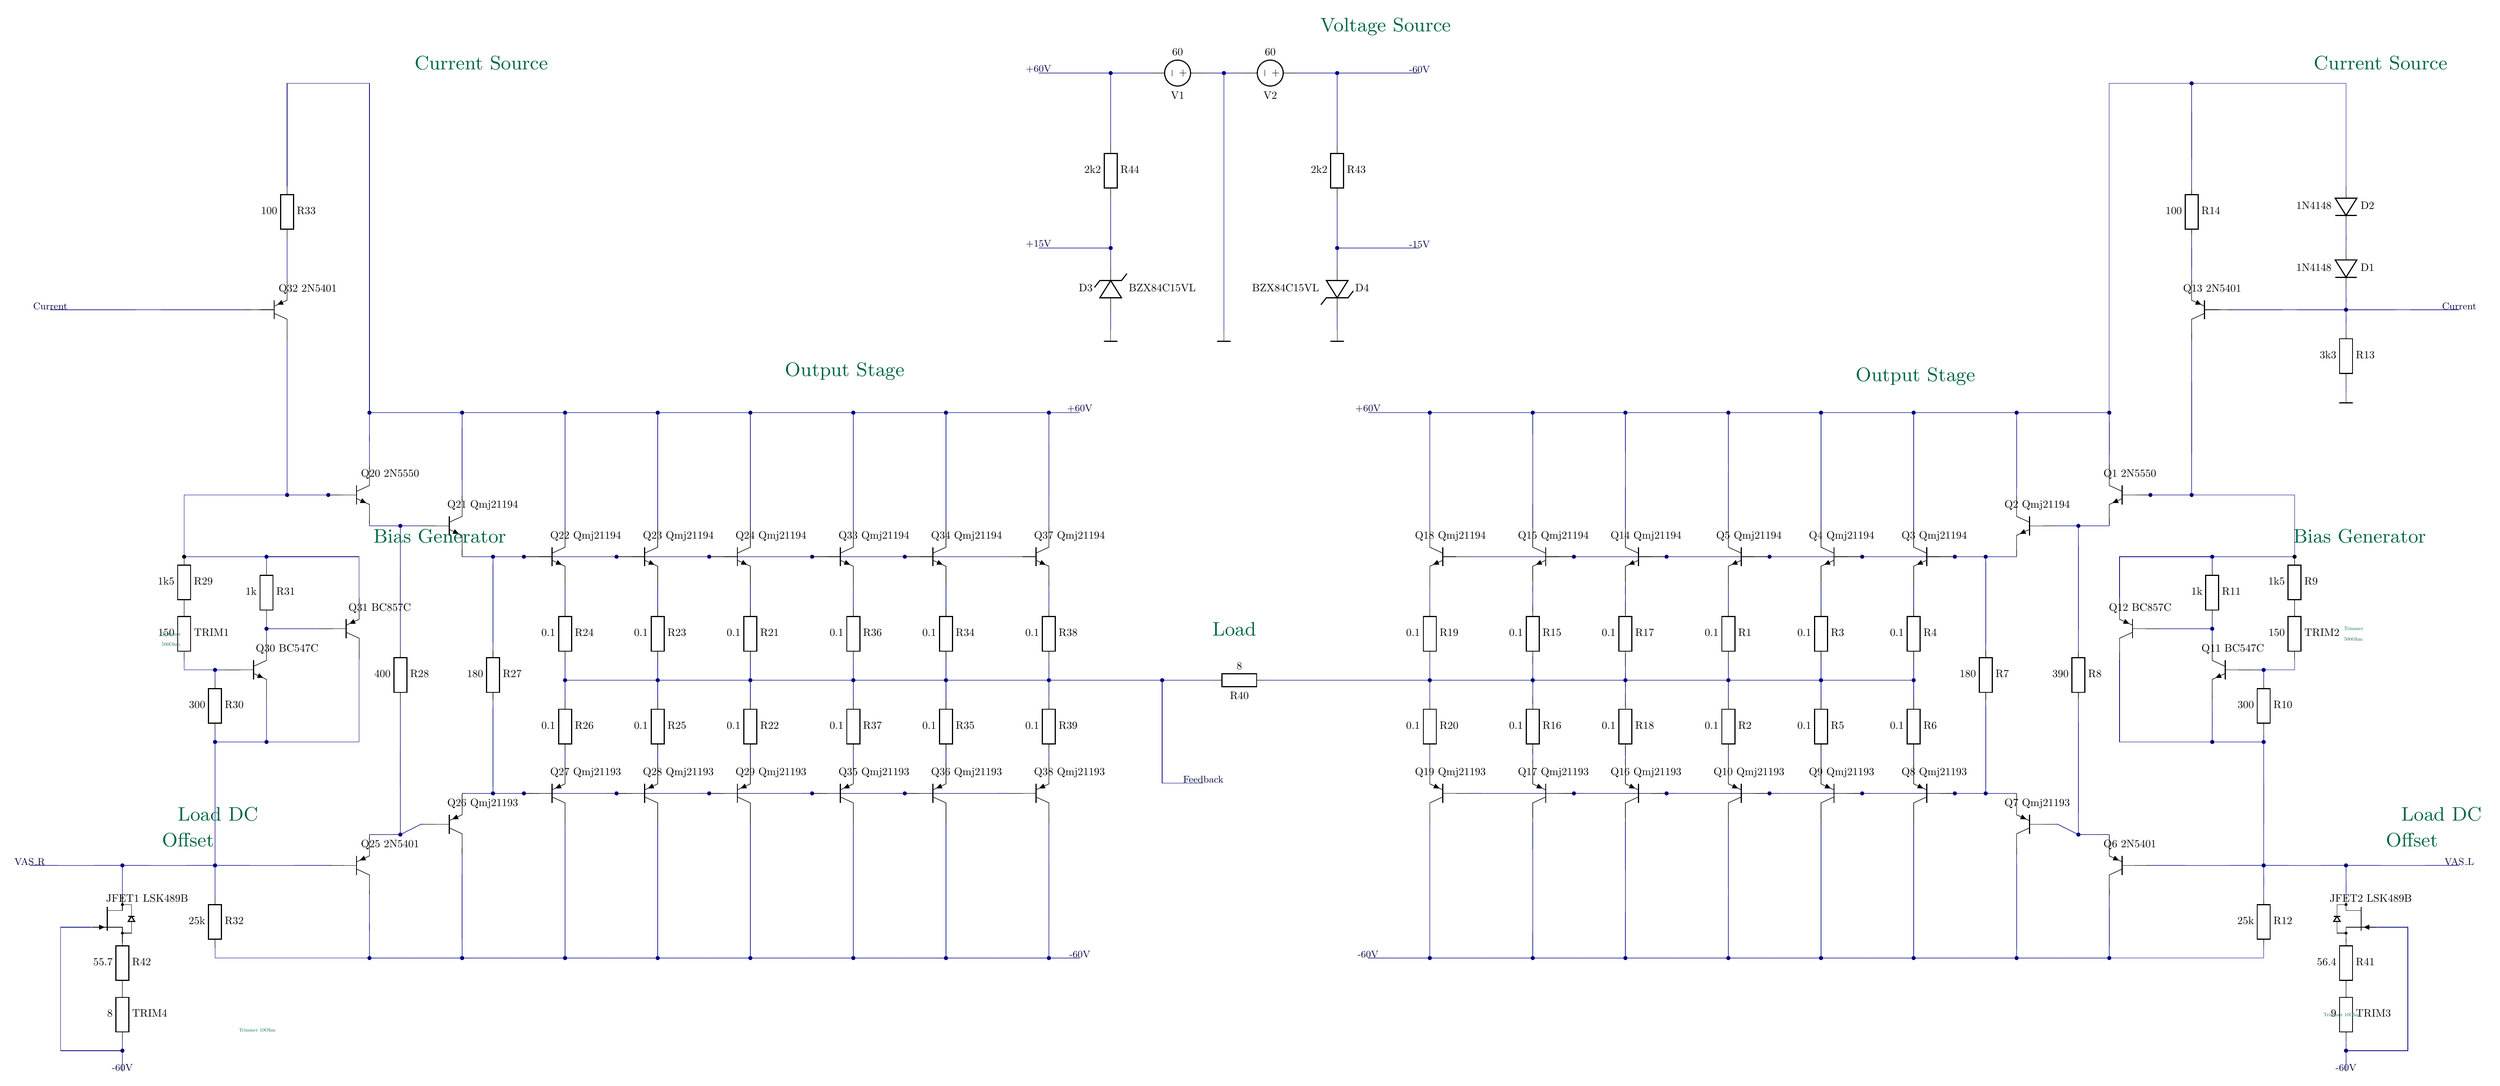
\begin{tikzpicture}[circuit ee IEC, scale=0.6666666667,line width=.5pt]% default: 0.4
	%\tikzstyle{every node}=[font=\small];%
	%\node [draw] at (0.0,0.0) {\pgfkeysvalueof{/tikz/circuitikz/tripoles/op amp/font}};
\draw [/lt2ti/Net](13.0,15.0)to[*short,*-, color=netcolor] (9.5,15.0);% wire w3
\draw [/lt2ti/Net](15.0,15.0)to[*short,-*, color=netcolor] (13.0,15.0);% wire w4
\draw [/lt2ti/Net](18.5,15.0)to[*short,*-, color=netcolor] (17.5,15.0);% wire w5
\draw [/lt2ti/Net](19.5,15.0)to[*short,-*, color=netcolor] (18.5,15.0);% wire w6
\draw [/lt2ti/Net](24.0,15.0)to[*short,*-, color=netcolor] (22.0,15.0);% wire w7
\draw [/lt2ti/Net](28.0,15.0)to[*short,-*, color=netcolor] (24.0,15.0);% wire w8
\draw [/lt2ti/Net](65.5,14.5)to[*short,*-, color=netcolor] (65.5,14.5);% wire w10_w51 start
\draw [/lt2ti/Net](61.5,-1.5)to[*short,-*, color=netcolor] (61.5,-1.5);% wire w10_w51 end
\draw [/lt2ti/Net](65.5,14.5) --  (61.5,14.5) -- (61.5,-1.5); % wire w10_w51 polyline 
\draw [/lt2ti/Net](13.0,11.5)to[*short,-*, color=netcolor] (13.0,15.0);% wire w12
\draw [/lt2ti/Net](24.0,11.5)to[*short,-*, color=netcolor] (24.0,15.0);% wire w13
\draw [/lt2ti/Net](-27.0,9.5)to[*short,-, color=netcolor] (-27.0,9.5);% wire w14_w9_w35 start
\draw [/lt2ti/Net](-23.0,-1.5)to[*short,-*, color=netcolor] (-23.0,-1.5);% wire w14_w9_w35 end
\draw [/lt2ti/Net](-27.0,9.5) --  (-27.0,14.5) --  (-23.0,14.5) -- (-23.0,-1.5); % wire w14_w9_w35 polyline 
\draw [/lt2ti/Net](65.5,9.5)to[*short,-*, color=netcolor] (65.5,14.5);% wire w15
\draw [/lt2ti/Net](73.0,9.5)to[*short,-, color=netcolor] (73.0,9.5);% wire w11_w16 start
\draw [/lt2ti/Net](65.5,14.5)to[*short,-*, color=netcolor] (65.5,14.5);% wire w11_w16 end
\draw [/lt2ti/Net](73.0,9.5) --  (73.0,14.5) -- (65.5,14.5); % wire w11_w16 polyline 
\draw [/lt2ti/Net](13.0,6.5)to[*short,*-, color=netcolor] (13.0,9.0);% wire w17
\draw [/lt2ti/Net](13.0,6.5)to[*short,*-, color=netcolor] (9.5,6.5);% wire w18
\draw [/lt2ti/Net](24.0,6.5)to[*short,*-, color=netcolor] (24.0,9.0);% wire w19
\draw [/lt2ti/Net](28.0,6.5)to[*short,-*, color=netcolor] (24.0,6.5);% wire w20
\draw [/lt2ti/Net](73.0,6.5)to[*short,-, color=netcolor] (73.0,7.5);% wire w21
\draw [/lt2ti/Net](13.0,5.5)to[*short,-*, color=netcolor] (13.0,6.5);% wire w22
\draw [/lt2ti/Net](24.0,5.5)to[*short,-*, color=netcolor] (24.0,6.5);% wire w23
\draw [/lt2ti/Net](-27.0,5.0)to[*short,-, color=netcolor] (-27.0,7.0);% wire w24
\draw [/lt2ti/Net](65.5,5.0)to[*short,-, color=netcolor] (65.5,7.0);% wire w25
\draw [/lt2ti/Net](-29.0,3.5)to[*short,-, color=netcolor] (-38.5,3.5);% wire w26
\draw [/lt2ti/Net](73.0,3.5)to[*short,*-, color=netcolor] (73.0,4.5);% wire w27
\draw [/lt2ti/Net](73.0,3.5)to[*short,*-, color=netcolor] (67.5,3.5);% wire w28
\draw [/lt2ti/Net](78.5,3.5)to[*short,-*, color=netcolor] (73.0,3.5);% wire w29
\draw [/lt2ti/Net](13.0,2.5)to[*short,-, color=netcolor] (13.0,3.5);% wire w30
\draw [/lt2ti/Net](18.5,2.5)to[*short,-*, color=netcolor] (18.5,15.0);% wire w31
\draw [/lt2ti/Net](24.0,2.5)to[*short,-, color=netcolor] (24.0,3.5);% wire w32
\draw [/lt2ti/Net](73.0,2.5)to[*short,-*, color=netcolor] (73.0,3.5);% wire w33
\draw [/lt2ti/Net](73.0,-0.5)to[*short,-, color=netcolor] (73.0,0.0);% wire w34
\draw [/lt2ti/Net](-18.5,-1.5)to[*short,*-*, color=netcolor] (-23.0,-1.5);% wire w36
\draw [/lt2ti/Net](-13.5,-1.5)to[*short,*-*, color=netcolor] (-18.5,-1.5);% wire w37
\draw [/lt2ti/Net](-9.0,-1.5)to[*short,*-*, color=netcolor] (-13.5,-1.5);% wire w38
\draw [/lt2ti/Net](-4.5,-1.5)to[*short,*-*, color=netcolor] (-9.0,-1.5);% wire w39
\draw [/lt2ti/Net](0.5,-1.5)to[*short,*-*, color=netcolor] (-4.5,-1.5);% wire w40
\draw [/lt2ti/Net](5.0,-1.5)to[*short,*-*, color=netcolor] (0.5,-1.5);% wire w41
\draw [/lt2ti/Net](10.0,-1.5)to[*short,*-*, color=netcolor] (5.0,-1.5);% wire w42
\draw [/lt2ti/Net](11.5,-1.5)to[*short,-*, color=netcolor] (10.0,-1.5);% wire w43
\draw [/lt2ti/Net](28.5,-1.5)to[*short,*-, color=netcolor] (25.5,-1.5);% wire w44
\draw [/lt2ti/Net](33.5,-1.5)to[*short,*-*, color=netcolor] (28.5,-1.5);% wire w45
\draw [/lt2ti/Net](38.0,-1.5)to[*short,*-*, color=netcolor] (33.5,-1.5);% wire w46
\draw [/lt2ti/Net](43.0,-1.5)to[*short,*-*, color=netcolor] (38.0,-1.5);% wire w47
\draw [/lt2ti/Net](47.5,-1.5)to[*short,*-*, color=netcolor] (43.0,-1.5);% wire w48
\draw [/lt2ti/Net](52.0,-1.5)to[*short,*-*, color=netcolor] (47.5,-1.5);% wire w49
\draw [/lt2ti/Net](57.0,-1.5)to[*short,*-*, color=netcolor] (52.0,-1.5);% wire w50
\draw [/lt2ti/Net](61.5,-1.5)to[*short,*-*, color=netcolor] (57.0,-1.5);% wire w52
\draw [/lt2ti/Net](-23.0,-4.0)to[*short,-*, color=netcolor] (-23.0,-1.5);% wire w53
\draw [/lt2ti/Net](61.5,-4.0)to[*short,-*, color=netcolor] (61.5,-1.5);% wire w54
\draw [/lt2ti/Net](-27.0,-5.5)to[*short,*-, color=netcolor] (-27.0,2.0);% wire w55
\draw [/lt2ti/Net](-27.0,-5.5)to[*short,*-, color=netcolor] (-27.0,-5.5);% wire w56_w81 start
\draw [/lt2ti/Net](-32.0,-8.5)to[*short,-*, color=netcolor] (-32.0,-8.5);% wire w56_w81 end
\draw [/lt2ti/Net](-27.0,-5.5) --  (-32.0,-5.5) -- (-32.0,-8.5); % wire w56_w81 polyline 
\draw [/lt2ti/Net](-25.0,-5.5)to[*short,*-*, color=netcolor] (-27.0,-5.5);% wire w57
\draw [/lt2ti/Net](-24.5,-5.5)to[*short,-*, color=netcolor] (-25.0,-5.5);% wire w58
\draw [/lt2ti/Net](-18.5,-5.5)to[*short,-*, color=netcolor] (-18.5,-1.5);% wire w59
\draw [/lt2ti/Net](57.0,-5.5)to[*short,-*, color=netcolor] (57.0,-1.5);% wire w60
\draw [/lt2ti/Net](63.5,-5.5)to[*short,*-, color=netcolor] (63.0,-5.5);% wire w61
\draw [/lt2ti/Net](65.5,-5.5)to[*short,*-, color=netcolor] (65.5,2.0);% wire w62
\draw [/lt2ti/Net](65.5,-5.5)to[*short,*-*, color=netcolor] (63.5,-5.5);% wire w63
\draw [/lt2ti/Net](-21.5,-7.0)to[*short,*-, color=netcolor] (-23.0,-7.0);% wire w65
\draw [/lt2ti/Net](-20.5,-7.0)to[*short,-*, color=netcolor] (-21.5,-7.0);% wire w66
\draw [/lt2ti/Net](-13.5,-7.0)to[*short,-*, color=netcolor] (-13.5,-1.5);% wire w67
\draw [/lt2ti/Net](-9.0,-7.0)to[*short,-*, color=netcolor] (-9.0,-1.5);% wire w68
\draw [/lt2ti/Net](-4.5,-7.0)to[*short,-*, color=netcolor] (-4.5,-1.5);% wire w69
\draw [/lt2ti/Net](0.5,-7.0)to[*short,-*, color=netcolor] (0.5,-1.5);% wire w70
\draw [/lt2ti/Net](5.0,-7.0)to[*short,-*, color=netcolor] (5.0,-1.5);% wire w71
\draw [/lt2ti/Net](10.0,-7.0)to[*short,-*, color=netcolor] (10.0,-1.5);% wire w72
\draw [/lt2ti/Net](28.5,-7.0)to[*short,-*, color=netcolor] (28.5,-1.5);% wire w73
\draw [/lt2ti/Net](33.5,-7.0)to[*short,-*, color=netcolor] (33.5,-1.5);% wire w74
\draw [/lt2ti/Net](38.0,-7.0)to[*short,-*, color=netcolor] (38.0,-1.5);% wire w75
\draw [/lt2ti/Net](43.0,-7.0)to[*short,-*, color=netcolor] (43.0,-1.5);% wire w76
\draw [/lt2ti/Net](47.5,-7.0)to[*short,-*, color=netcolor] (47.5,-1.5);% wire w77
\draw [/lt2ti/Net](52.0,-7.0)to[*short,-*, color=netcolor] (52.0,-1.5);% wire w78
\draw [/lt2ti/Net](60.0,-7.0)to[*short,*-, color=netcolor] (59.0,-7.0);% wire w79
\draw [/lt2ti/Net](61.5,-7.0)to[*short,-*, color=netcolor] (60.0,-7.0);% wire w80
\draw [/lt2ti/Net](-28.0,-8.5)to[*short,*-*, color=netcolor] (-32.0,-8.5);% wire w82
\draw [/lt2ti/Net](-17.0,-8.5)to[*short,*-, color=netcolor] (-18.5,-8.5);% wire w84
\draw [/lt2ti/Net](-15.5,-8.5)to[*short,*-*, color=netcolor] (-17.0,-8.5);% wire w85
\draw [/lt2ti/Net](-11.0,-8.5)to[*short,*-*, color=netcolor] (-15.5,-8.5);% wire w86
\draw [/lt2ti/Net](-6.5,-8.5)to[*short,*-*, color=netcolor] (-11.0,-8.5);% wire w87
\draw [/lt2ti/Net](-1.5,-8.5)to[*short,*-*, color=netcolor] (-6.5,-8.5);% wire w88
\draw [/lt2ti/Net](3.0,-8.5)to[*short,*-*, color=netcolor] (-1.5,-8.5);% wire w89
\draw [/lt2ti/Net](8.0,-8.5)to[*short,-*, color=netcolor] (3.0,-8.5);% wire w90
\draw [/lt2ti/Net](35.5,-8.5)to[*short,*-, color=netcolor] (30.5,-8.5);% wire w91
\draw [/lt2ti/Net](40.0,-8.5)to[*short,*-*, color=netcolor] (35.5,-8.5);% wire w92
\draw [/lt2ti/Net](45.0,-8.5)to[*short,*-*, color=netcolor] (40.0,-8.5);% wire w93
\draw [/lt2ti/Net](49.5,-8.5)to[*short,*-*, color=netcolor] (45.0,-8.5);% wire w94
\draw [/lt2ti/Net](54.0,-8.5)to[*short,*-*, color=netcolor] (49.5,-8.5);% wire w95
\draw [/lt2ti/Net](55.5,-8.5)to[*short,*-*, color=netcolor] (54.0,-8.5);% wire w96
\draw [/lt2ti/Net](57.0,-8.5)to[*short,-*, color=netcolor] (55.5,-8.5);% wire w97
\draw [/lt2ti/Net](66.5,-8.5)to[*short,*-, color=netcolor] (66.5,-8.5);% wire w98_w104 start
\draw [/lt2ti/Net](62.0,-10.5)to[*short,-, color=netcolor] (62.0,-10.5);% wire w98_w104 end
\draw [/lt2ti/Net](66.5,-8.5) --  (62.0,-8.5) -- (62.0,-10.5); % wire w98_w104 polyline 
\draw [/lt2ti/Net](70.5,-8.5)to[*short,*-*, color=netcolor] (66.5,-8.5);% wire w100
\draw [/lt2ti/Net](70.5,-8.5)to[*short,*-, color=netcolor] (70.5,-8.5);% wire w64_w99 start
\draw [/lt2ti/Net](65.5,-5.5)to[*short,-*, color=netcolor] (65.5,-5.5);% wire w64_w99 end
\draw [/lt2ti/Net](70.5,-8.5) --  (70.5,-5.5) -- (65.5,-5.5); % wire w64_w99 polyline 
\draw [/lt2ti/Net](-28.0,-9.0)to[*short,-*, color=netcolor] (-28.0,-8.5);% wire w101
\draw [/lt2ti/Net](66.5,-9.0)to[*short,-*, color=netcolor] (66.5,-8.5);% wire w102
\draw [/lt2ti/Net](-23.5,-10.5)to[*short,-, color=netcolor] (-23.5,-10.5);% wire w83_w103 start
\draw [/lt2ti/Net](-28.0,-8.5)to[*short,-*, color=netcolor] (-28.0,-8.5);% wire w83_w103 end
\draw [/lt2ti/Net](-23.5,-10.5) --  (-23.5,-8.5) -- (-28.0,-8.5); % wire w83_w103 polyline 
\draw [/lt2ti/Net](-13.5,-11.0)to[*short,-, color=netcolor] (-13.5,-10.0);% wire w105
\draw [/lt2ti/Net](-9.0,-11.0)to[*short,-, color=netcolor] (-9.0,-10.0);% wire w106
\draw [/lt2ti/Net](-4.5,-11.0)to[*short,-, color=netcolor] (-4.5,-10.0);% wire w107
\draw [/lt2ti/Net](0.5,-11.0)to[*short,-, color=netcolor] (0.5,-10.0);% wire w108
\draw [/lt2ti/Net](5.0,-11.0)to[*short,-, color=netcolor] (5.0,-10.0);% wire w109
\draw [/lt2ti/Net](10.0,-11.0)to[*short,-, color=netcolor] (10.0,-10.0);% wire w110
\draw [/lt2ti/Net](28.5,-11.0)to[*short,-, color=netcolor] (28.5,-10.0);% wire w111
\draw [/lt2ti/Net](33.5,-11.0)to[*short,-, color=netcolor] (33.5,-10.0);% wire w112
\draw [/lt2ti/Net](38.0,-11.0)to[*short,-, color=netcolor] (38.0,-10.0);% wire w113
\draw [/lt2ti/Net](43.0,-11.0)to[*short,-, color=netcolor] (43.0,-10.0);% wire w114
\draw [/lt2ti/Net](47.5,-11.0)to[*short,-, color=netcolor] (47.5,-10.0);% wire w115
\draw [/lt2ti/Net](52.0,-11.0)to[*short,-, color=netcolor] (52.0,-10.0);% wire w116
\draw [/lt2ti/Net](-28.0,-12.0)to[*short,*-, color=netcolor] (-28.0,-11.5);% wire w117
\draw [/lt2ti/Net](-25.5,-12.0)to[*short,-*, color=netcolor] (-28.0,-12.0);% wire w118
\draw [/lt2ti/Net](66.5,-12.0)to[*short,*-, color=netcolor] (66.5,-11.5);% wire w119
\draw [/lt2ti/Net](66.5,-12.0)to[*short,*-, color=netcolor] (64.0,-12.0);% wire w120
\draw [/lt2ti/Net](-28.0,-12.5)to[*short,-*, color=netcolor] (-28.0,-12.0);% wire w121
\draw [/lt2ti/Net](66.5,-12.5)to[*short,-*, color=netcolor] (66.5,-12.0);% wire w122
\draw [/lt2ti/Net](-21.5,-13.0)to[*short,-*, color=netcolor] (-21.5,-7.0);% wire w123
\draw [/lt2ti/Net](-17.0,-13.0)to[*short,-*, color=netcolor] (-17.0,-8.5);% wire w124
\draw [/lt2ti/Net](55.5,-13.0)to[*short,-*, color=netcolor] (55.5,-8.5);% wire w125
\draw [/lt2ti/Net](60.0,-13.0)to[*short,-*, color=netcolor] (60.0,-7.0);% wire w126
\draw [/lt2ti/Net](-30.5,-14.0)to[*short,*-, color=netcolor] (-30.5,-14.0);% wire w127_w128 start
\draw [/lt2ti/Net](-32.0,-13.5)to[*short,-, color=netcolor] (-32.0,-13.5);% wire w127_w128 end
\draw [/lt2ti/Net](-30.5,-14.0) --  (-32.0,-14.0) -- (-32.0,-13.5); % wire w127_w128 polyline 
\draw [/lt2ti/Net](-30.0,-14.0)to[*short,-*, color=netcolor] (-30.5,-14.0);% wire w129
\draw [/lt2ti/Net](69.0,-14.0)to[*short,*-, color=netcolor] (68.5,-14.0);% wire w130
\draw [/lt2ti/Net](70.5,-13.5)to[*short,-, color=netcolor] (70.5,-13.5);% wire w131_w132 start
\draw [/lt2ti/Net](69.0,-14.0)to[*short,-*, color=netcolor] (69.0,-14.0);% wire w131_w132 end
\draw [/lt2ti/Net](70.5,-13.5) --  (70.5,-14.0) -- (69.0,-14.0); % wire w131_w132 polyline 
\draw [/lt2ti/Net](-30.5,-14.5)to[*short,-*, color=netcolor] (-30.5,-14.0);% wire w133
\draw [/lt2ti/Net](-13.5,-14.5)to[*short,*-, color=netcolor] (-13.5,-13.5);% wire w134
\draw [/lt2ti/Net](-9.0,-14.5)to[*short,*-, color=netcolor] (-9.0,-13.5);% wire w135
\draw [/lt2ti/Net](-9.0,-14.5)to[*short,*-*, color=netcolor] (-13.5,-14.5);% wire w136
\draw [/lt2ti/Net](-4.5,-14.5)to[*short,*-, color=netcolor] (-4.5,-13.5);% wire w137
\draw [/lt2ti/Net](-4.5,-14.5)to[*short,*-*, color=netcolor] (-9.0,-14.5);% wire w138
\draw [/lt2ti/Net](0.5,-14.5)to[*short,*-, color=netcolor] (0.5,-13.5);% wire w139
\draw [/lt2ti/Net](0.5,-14.5)to[*short,*-*, color=netcolor] (-4.5,-14.5);% wire w140
\draw [/lt2ti/Net](5.0,-14.5)to[*short,*-, color=netcolor] (5.0,-13.5);% wire w141
\draw [/lt2ti/Net](5.0,-14.5)to[*short,*-*, color=netcolor] (0.5,-14.5);% wire w142
\draw [/lt2ti/Net](10.0,-14.5)to[*short,*-, color=netcolor] (10.0,-13.5);% wire w143
\draw [/lt2ti/Net](10.0,-14.5)to[*short,*-*, color=netcolor] (5.0,-14.5);% wire w144
\draw [/lt2ti/Net](15.5,-14.5)to[*short,*-*, color=netcolor] (10.0,-14.5);% wire w145
\draw [/lt2ti/Net](18.0,-14.5)to[*short,-*, color=netcolor] (15.5,-14.5);% wire w146
\draw [/lt2ti/Net](28.5,-14.5)to[*short,*-, color=netcolor] (28.5,-13.5);% wire w147
\draw [/lt2ti/Net](28.5,-14.5)to[*short,*-, color=netcolor] (20.5,-14.5);% wire w148
\draw [/lt2ti/Net](33.5,-14.5)to[*short,*-, color=netcolor] (33.5,-13.5);% wire w149
\draw [/lt2ti/Net](33.5,-14.5)to[*short,*-*, color=netcolor] (28.5,-14.5);% wire w150
\draw [/lt2ti/Net](38.0,-14.5)to[*short,*-, color=netcolor] (38.0,-13.5);% wire w151
\draw [/lt2ti/Net](38.0,-14.5)to[*short,*-*, color=netcolor] (33.5,-14.5);% wire w152
\draw [/lt2ti/Net](43.0,-14.5)to[*short,*-, color=netcolor] (43.0,-13.5);% wire w153
\draw [/lt2ti/Net](43.0,-14.5)to[*short,*-*, color=netcolor] (38.0,-14.5);% wire w154
\draw [/lt2ti/Net](47.5,-14.5)to[*short,*-, color=netcolor] (47.5,-13.5);% wire w155
\draw [/lt2ti/Net](47.5,-14.5)to[*short,*-*, color=netcolor] (43.0,-14.5);% wire w156
\draw [/lt2ti/Net](52.0,-14.5)to[*short,*-, color=netcolor] (52.0,-13.5);% wire w157
\draw [/lt2ti/Net](52.0,-14.5)to[*short,*-*, color=netcolor] (47.5,-14.5);% wire w158
\draw [/lt2ti/Net](69.0,-14.5)to[*short,-*, color=netcolor] (69.0,-14.0);% wire w159
\draw [/lt2ti/Net](-13.5,-15.5)to[*short,-*, color=netcolor] (-13.5,-14.5);% wire w160
\draw [/lt2ti/Net](-9.0,-15.5)to[*short,-*, color=netcolor] (-9.0,-14.5);% wire w161
\draw [/lt2ti/Net](-4.5,-15.5)to[*short,-*, color=netcolor] (-4.5,-14.5);% wire w162
\draw [/lt2ti/Net](0.5,-15.5)to[*short,-*, color=netcolor] (0.5,-14.5);% wire w163
\draw [/lt2ti/Net](5.0,-15.5)to[*short,-*, color=netcolor] (5.0,-14.5);% wire w164
\draw [/lt2ti/Net](10.0,-15.5)to[*short,-*, color=netcolor] (10.0,-14.5);% wire w165
\draw [/lt2ti/Net](28.5,-15.5)to[*short,-*, color=netcolor] (28.5,-14.5);% wire w166
\draw [/lt2ti/Net](33.5,-15.5)to[*short,-*, color=netcolor] (33.5,-14.5);% wire w167
\draw [/lt2ti/Net](38.0,-15.5)to[*short,-*, color=netcolor] (38.0,-14.5);% wire w168
\draw [/lt2ti/Net](43.0,-15.5)to[*short,-*, color=netcolor] (43.0,-14.5);% wire w169
\draw [/lt2ti/Net](47.5,-15.5)to[*short,-*, color=netcolor] (47.5,-14.5);% wire w170
\draw [/lt2ti/Net](52.0,-15.5)to[*short,-*, color=netcolor] (52.0,-14.5);% wire w171
\draw [/lt2ti/Net](-30.5,-17.5)to[*short,*-, color=netcolor] (-30.5,-17.0);% wire w172
\draw [/lt2ti/Net](-28.0,-17.5)to[*short,*-, color=netcolor] (-28.0,-15.5);% wire w173
\draw [/lt2ti/Net](-28.0,-17.5)to[*short,*-*, color=netcolor] (-30.5,-17.5);% wire w174
\draw [/lt2ti/Net](-23.5,-13.5)to[*short,-, color=netcolor] (-23.5,-13.5);% wire w175_w176 start
\draw [/lt2ti/Net](-28.0,-17.5)to[*short,-*, color=netcolor] (-28.0,-17.5);% wire w175_w176 end
\draw [/lt2ti/Net](-23.5,-13.5) --  (-23.5,-17.5) -- (-28.0,-17.5); % wire w175_w176 polyline 
\draw [/lt2ti/Net](66.5,-17.5)to[*short,*-, color=netcolor] (66.5,-15.5);% wire w178
\draw [/lt2ti/Net](66.5,-17.5)to[*short,*-, color=netcolor] (66.5,-17.5);% wire w177_w179 start
\draw [/lt2ti/Net](62.0,-13.5)to[*short,-, color=netcolor] (62.0,-13.5);% wire w177_w179 end
\draw [/lt2ti/Net](66.5,-17.5) --  (62.0,-17.5) -- (62.0,-13.5); % wire w177_w179 polyline 
\draw [/lt2ti/Net](69.0,-17.5)to[*short,*-, color=netcolor] (69.0,-17.0);% wire w180
\draw [/lt2ti/Net](69.0,-17.5)to[*short,*-*, color=netcolor] (66.5,-17.5);% wire w181
\draw [/lt2ti/Net](-13.5,-18.5)to[*short,-, color=netcolor] (-13.5,-18.0);% wire w182
\draw [/lt2ti/Net](-9.0,-18.5)to[*short,-, color=netcolor] (-9.0,-18.0);% wire w183
\draw [/lt2ti/Net](-4.5,-18.5)to[*short,-, color=netcolor] (-4.5,-18.0);% wire w184
\draw [/lt2ti/Net](0.5,-18.5)to[*short,-, color=netcolor] (0.5,-18.0);% wire w185
\draw [/lt2ti/Net](5.0,-18.5)to[*short,-, color=netcolor] (5.0,-18.0);% wire w186
\draw [/lt2ti/Net](10.0,-18.5)to[*short,-, color=netcolor] (10.0,-18.0);% wire w187
\draw [/lt2ti/Net](28.5,-18.5)to[*short,-, color=netcolor] (28.5,-18.0);% wire w188
\draw [/lt2ti/Net](33.5,-18.5)to[*short,-, color=netcolor] (33.5,-18.0);% wire w189
\draw [/lt2ti/Net](38.0,-18.5)to[*short,-, color=netcolor] (38.0,-18.0);% wire w190
\draw [/lt2ti/Net](43.0,-18.5)to[*short,-, color=netcolor] (43.0,-18.0);% wire w191
\draw [/lt2ti/Net](47.5,-18.5)to[*short,-, color=netcolor] (47.5,-18.0);% wire w192
\draw [/lt2ti/Net](52.0,-18.5)to[*short,-, color=netcolor] (52.0,-18.0);% wire w193
\draw [/lt2ti/Net](17.5,-19.5)to[*short,-, color=netcolor] (17.5,-19.5);% wire w194_w195 start
\draw [/lt2ti/Net](15.5,-14.5)to[*short,-*, color=netcolor] (15.5,-14.5);% wire w194_w195 end
\draw [/lt2ti/Net](17.5,-19.5) --  (15.5,-19.5) -- (15.5,-14.5); % wire w194_w195 polyline 
\draw [/lt2ti/Net](-17.0,-20.0)to[*short,*-, color=netcolor] (-17.0,-15.5);% wire w196
\draw [/lt2ti/Net](-17.0,-20.0)to[*short,*-, color=netcolor] (-18.5,-20.0);% wire w197
\draw [/lt2ti/Net](-15.5,-20.0)to[*short,*-*, color=netcolor] (-17.0,-20.0);% wire w198
\draw [/lt2ti/Net](-11.0,-20.0)to[*short,*-*, color=netcolor] (-15.5,-20.0);% wire w199
\draw [/lt2ti/Net](-6.5,-20.0)to[*short,*-*, color=netcolor] (-11.0,-20.0);% wire w200
\draw [/lt2ti/Net](-1.5,-20.0)to[*short,*-*, color=netcolor] (-6.5,-20.0);% wire w201
\draw [/lt2ti/Net](3.0,-20.0)to[*short,*-*, color=netcolor] (-1.5,-20.0);% wire w202
\draw [/lt2ti/Net](8.0,-20.0)to[*short,-*, color=netcolor] (3.0,-20.0);% wire w203
\draw [/lt2ti/Net](35.5,-20.0)to[*short,*-, color=netcolor] (30.5,-20.0);% wire w204
\draw [/lt2ti/Net](40.0,-20.0)to[*short,*-*, color=netcolor] (35.5,-20.0);% wire w205
\draw [/lt2ti/Net](45.0,-20.0)to[*short,*-*, color=netcolor] (40.0,-20.0);% wire w206
\draw [/lt2ti/Net](49.5,-20.0)to[*short,*-*, color=netcolor] (45.0,-20.0);% wire w207
\draw [/lt2ti/Net](54.0,-20.0)to[*short,*-*, color=netcolor] (49.5,-20.0);% wire w208
\draw [/lt2ti/Net](55.5,-20.0)to[*short,*-, color=netcolor] (55.5,-15.5);% wire w209
\draw [/lt2ti/Net](55.5,-20.0)to[*short,*-*, color=netcolor] (54.0,-20.0);% wire w210
\draw [/lt2ti/Net](57.0,-20.0)to[*short,-*, color=netcolor] (55.5,-20.0);% wire w211
\draw [/lt2ti/Net](-21.5,-22.0)to[*short,*-, color=netcolor] (-21.5,-15.5);% wire w212
\draw [/lt2ti/Net](-21.5,-22.0)to[*short,*-, color=netcolor] (-20.5,-21.5);% wire w213
\draw [/lt2ti/Net](-21.5,-22.0)to[*short,*-, color=netcolor] (-23.0,-22.0);% wire w214
\draw [/lt2ti/Net](60.0,-22.0)to[*short,*-, color=netcolor] (60.0,-15.5);% wire w215
\draw [/lt2ti/Net](60.0,-22.0)to[*short,*-, color=netcolor] (59.0,-21.5);% wire w216
\draw [/lt2ti/Net](61.5,-22.0)to[*short,-*, color=netcolor] (60.0,-22.0);% wire w217
\draw [/lt2ti/Net](-35.0,-23.5)to[*short,*-, color=netcolor] (-39.5,-23.5);% wire w218
\draw [/lt2ti/Net](-30.5,-23.5)to[*short,*-*, color=netcolor] (-30.5,-17.5);% wire w219
\draw [/lt2ti/Net](-30.5,-23.5)to[*short,*-*, color=netcolor] (-35.0,-23.5);% wire w220
\draw [/lt2ti/Net](-25.0,-23.5)to[*short,-*, color=netcolor] (-30.5,-23.5);% wire w221
\draw [/lt2ti/Net](69.0,-23.5)to[*short,*-*, color=netcolor] (69.0,-17.5);% wire w222
\draw [/lt2ti/Net](69.0,-23.5)to[*short,*-, color=netcolor] (63.5,-23.5);% wire w223
\draw [/lt2ti/Net](73.0,-23.5)to[*short,*-*, color=netcolor] (69.0,-23.5);% wire w224
\draw [/lt2ti/Net](78.5,-23.5)to[*short,-*, color=netcolor] (73.0,-23.5);% wire w225
\draw [/lt2ti/Net](-35.0,-24.0)to[*short,-*, color=netcolor] (-35.0,-23.5);% wire w226
\draw [/lt2ti/Net](73.0,-24.0)to[*short,-*, color=netcolor] (73.0,-23.5);% wire w227
\draw [/lt2ti/Net](-30.5,-25.0)to[*short,-*, color=netcolor] (-30.5,-23.5);% wire w228
\draw [/lt2ti/Net](69.0,-25.0)to[*short,-*, color=netcolor] (69.0,-23.5);% wire w229
\draw [/lt2ti/Net](-23.0,-28.0)to[*short,*-, color=netcolor] (-23.0,-25.0);% wire w233
\draw [/lt2ti/Net](-23.0,-28.0)to[*short,*-, color=netcolor] (-23.0,-28.0);% wire w232_w234 start
\draw [/lt2ti/Net](-30.5,-27.5)to[*short,-, color=netcolor] (-30.5,-27.5);% wire w232_w234 end
\draw [/lt2ti/Net](-23.0,-28.0) --  (-30.5,-28.0) -- (-30.5,-27.5); % wire w232_w234 polyline 
\draw [/lt2ti/Net](-18.5,-28.0)to[*short,*-, color=netcolor] (-18.5,-23.0);% wire w235
\draw [/lt2ti/Net](-18.5,-28.0)to[*short,*-*, color=netcolor] (-23.0,-28.0);% wire w236
\draw [/lt2ti/Net](-13.5,-28.0)to[*short,*-, color=netcolor] (-13.5,-21.5);% wire w237
\draw [/lt2ti/Net](-13.5,-28.0)to[*short,*-*, color=netcolor] (-18.5,-28.0);% wire w238
\draw [/lt2ti/Net](-9.0,-28.0)to[*short,*-, color=netcolor] (-9.0,-21.5);% wire w239
\draw [/lt2ti/Net](-9.0,-28.0)to[*short,*-*, color=netcolor] (-13.5,-28.0);% wire w240
\draw [/lt2ti/Net](-4.5,-28.0)to[*short,*-, color=netcolor] (-4.5,-21.5);% wire w241
\draw [/lt2ti/Net](-4.5,-28.0)to[*short,*-*, color=netcolor] (-9.0,-28.0);% wire w242
\draw [/lt2ti/Net](0.5,-28.0)to[*short,*-, color=netcolor] (0.5,-21.5);% wire w243
\draw [/lt2ti/Net](0.5,-28.0)to[*short,*-*, color=netcolor] (-4.5,-28.0);% wire w244
\draw [/lt2ti/Net](5.0,-28.0)to[*short,*-, color=netcolor] (5.0,-21.5);% wire w245
\draw [/lt2ti/Net](5.0,-28.0)to[*short,*-*, color=netcolor] (0.5,-28.0);% wire w246
\draw [/lt2ti/Net](10.0,-28.0)to[*short,*-, color=netcolor] (10.0,-21.5);% wire w247
\draw [/lt2ti/Net](10.0,-28.0)to[*short,*-*, color=netcolor] (5.0,-28.0);% wire w248
\draw [/lt2ti/Net](11.5,-28.0)to[*short,-*, color=netcolor] (10.0,-28.0);% wire w249
\draw [/lt2ti/Net](28.5,-28.0)to[*short,*-, color=netcolor] (28.5,-21.5);% wire w250
\draw [/lt2ti/Net](28.5,-28.0)to[*short,*-, color=netcolor] (25.5,-28.0);% wire w251
\draw [/lt2ti/Net](33.5,-28.0)to[*short,*-, color=netcolor] (33.5,-21.5);% wire w252
\draw [/lt2ti/Net](33.5,-28.0)to[*short,*-*, color=netcolor] (28.5,-28.0);% wire w253
\draw [/lt2ti/Net](38.0,-28.0)to[*short,*-, color=netcolor] (38.0,-21.5);% wire w254
\draw [/lt2ti/Net](38.0,-28.0)to[*short,*-*, color=netcolor] (33.5,-28.0);% wire w255
\draw [/lt2ti/Net](43.0,-28.0)to[*short,*-, color=netcolor] (43.0,-21.5);% wire w256
\draw [/lt2ti/Net](43.0,-28.0)to[*short,*-*, color=netcolor] (38.0,-28.0);% wire w257
\draw [/lt2ti/Net](47.5,-28.0)to[*short,*-, color=netcolor] (47.5,-21.5);% wire w258
\draw [/lt2ti/Net](47.5,-28.0)to[*short,*-*, color=netcolor] (43.0,-28.0);% wire w259
\draw [/lt2ti/Net](52.0,-28.0)to[*short,*-, color=netcolor] (52.0,-21.5);% wire w260
\draw [/lt2ti/Net](52.0,-28.0)to[*short,*-*, color=netcolor] (47.5,-28.0);% wire w261
\draw [/lt2ti/Net](57.0,-28.0)to[*short,*-, color=netcolor] (57.0,-23.0);% wire w262
\draw [/lt2ti/Net](57.0,-28.0)to[*short,*-*, color=netcolor] (52.0,-28.0);% wire w263
\draw [/lt2ti/Net](61.5,-28.0)to[*short,*-, color=netcolor] (61.5,-25.0);% wire w264
\draw [/lt2ti/Net](61.5,-28.0)to[*short,*-*, color=netcolor] (57.0,-28.0);% wire w265
\draw [/lt2ti/Net](69.0,-27.5)to[*short,-, color=netcolor] (69.0,-27.5);% wire w266_w267 start
\draw [/lt2ti/Net](61.5,-28.0)to[*short,-*, color=netcolor] (61.5,-28.0);% wire w266_w267 end
\draw [/lt2ti/Net](69.0,-27.5) --  (69.0,-28.0) -- (61.5,-28.0); % wire w266_w267 polyline 
\draw [/lt2ti/Net](-35.0,-32.5)to[*short,*-, color=netcolor] (-35.0,-32.0);% wire w269
\draw [/lt2ti/Net](-35.0,-32.5)to[*short,*-, color=netcolor] (-35.0,-32.5);% wire w270_w230_w268 start
\draw [/lt2ti/Net](-36.5,-26.5)to[*short,-, color=netcolor] (-36.5,-26.5);% wire w270_w230_w268 end
\draw [/lt2ti/Net](-35.0,-32.5) --  (-38.0,-32.5) --  (-38.0,-26.5) -- (-36.5,-26.5); % wire w270_w230_w268 polyline 
\draw [/lt2ti/Net](73.0,-32.5)to[*short,*-, color=netcolor] (73.0,-32.0);% wire w271
\draw [/lt2ti/Net](73.0,-32.5)to[*short,*-, color=netcolor] (73.0,-32.5);% wire w273_w231_w272 start
\draw [/lt2ti/Net](74.5,-26.5)to[*short,-, color=netcolor] (74.5,-26.5);% wire w273_w231_w272 end
\draw [/lt2ti/Net](73.0,-32.5) --  (76.0,-32.5) --  (76.0,-26.5) -- (74.5,-26.5); % wire w273_w231_w272 polyline 
\draw [/lt2ti/Net](-35.0,-33.5)to[*short,-*, color=netcolor] (-35.0,-32.5);% wire w274
\draw [/lt2ti/Net](73.0,-33.5)to[*short,-*, color=netcolor] (73.0,-32.5);% wire w275
 \draw (18.5, 2.5) node[rground, xscale=1, yscale=1, rotate=0, ] (undefined) {};%  (undefined)++(0.0,0.0) node {undefined }; % component "circuiTikz\gnd" "undefined" 
 \draw (73.0, -0.5) node[rground, xscale=1, yscale=1, rotate=0, ] (undefined) {};%  (undefined)++(0.0,0.0) node {undefined }; % component "circuiTikz\gnd" "undefined" 
 \draw (13.0, 2.5) node[rground, xscale=1, yscale=1, rotate=0, ] (undefined) {};%  (undefined)++(0.0,0.0) node {undefined }; % component "circuiTikz\gnd" "undefined" 
 \draw (24.0, 2.5) node[rground, xscale=1, yscale=1, rotate=0, ] (undefined) {};%  (undefined)++(0.0,0.0) node {undefined }; % component "circuiTikz\gnd" "undefined" 
  \draw (15.0, 15.0) to[*V, l_=V1, a^=60,invert, -, ] (17.5,15.0){}; % component "voltage" "V1" 
  \draw (19.5, 15.0) to[*V, l_=V2, a^=60,invert, -, ] (22.0,15.0){}; % component "voltage" "V2" 
 \draw (61.5, -5.5) node[npn, nobodydiode, xscale=-1, rotate=0, ] (Q1) {}   (Q1)++(1.0,1) node {Q1 2N5550}; % component "npn" "Q1" 
 \draw (63.5, -5.5) to [*short, -] (Q1.B); \draw (61.5, -7.0) to [*short, -] (Q1.E); \draw (61.5, -4.0) to [*short, -] (Q1.C);% extend wires to the connection points   % component "npn" "Q1" 
 \draw (57.0, -7.0) node[npn, nobodydiode, xscale=-1, rotate=0, ] (Q2) {}   (Q2)++(1.0,1) node {Q2 Qmj21194}; % component "npn" "Q2" 
 \draw (59.0, -7.0) to [*short, -] (Q2.B); \draw (57.0, -8.5) to [*short, -] (Q2.E); \draw (57.0, -5.5) to [*short, -] (Q2.C);% extend wires to the connection points   % component "npn" "Q2" 
 \draw (52.0, -8.5) node[npn, nobodydiode, xscale=-1, rotate=0, ] (Q3) {}   (Q3)++(1.0,1) node {Q3 Qmj21194}; % component "npn" "Q3" 
 \draw (54.0, -8.5) to [*short, -] (Q3.B); \draw (52.0, -10.0) to [*short, -] (Q3.E); \draw (52.0, -7.0) to [*short, -] (Q3.C);% extend wires to the connection points   % component "npn" "Q3" 
 \draw (47.5, -8.5) node[npn, nobodydiode, xscale=-1, rotate=0, ] (Q4) {}   (Q4)++(1.0,1) node {Q4 Qmj21194}; % component "npn" "Q4" 
 \draw (49.5, -8.5) to [*short, -] (Q4.B); \draw (47.5, -10.0) to [*short, -] (Q4.E); \draw (47.5, -7.0) to [*short, -] (Q4.C);% extend wires to the connection points   % component "npn" "Q4" 
 \draw (43.0, -8.5) node[npn, nobodydiode, xscale=-1, rotate=0, ] (Q5) {}   (Q5)++(1.0,1) node {Q5 Qmj21194}; % component "npn" "Q5" 
 \draw (45.0, -8.5) to [*short, -] (Q5.B); \draw (43.0, -10.0) to [*short, -] (Q5.E); \draw (43.0, -7.0) to [*short, -] (Q5.C);% extend wires to the connection points   % component "npn" "Q5" 
 \draw (61.5, -23.5) node[pnp, nobodydiode, xscale=-1, yscale=1, rotate=-360, ] (Q6) {}   (Q6)++(1.0,1) node {Q6 2N5401}; % component "pnp" "Q6" 
 \draw (63.5, -23.5) to [*short, -] (Q6.B); \draw (61.5, -22.0) to [*short, -] (Q6.E); \draw (61.5, -25.0) to [*short, -] (Q6.C);% extend wires to the connection points   % component "pnp" "Q6" 
 \draw (57.0, -21.5) node[pnp, nobodydiode, xscale=-1, yscale=1, rotate=-360, ] (Q7) {}   (Q7)++(1.0,1) node {Q7 Qmj21193}; % component "pnp" "Q7" 
 \draw (59.0, -21.5) to [*short, -] (Q7.B); \draw (57.0, -20.0) to [*short, -] (Q7.E); \draw (57.0, -23.0) to [*short, -] (Q7.C);% extend wires to the connection points   % component "pnp" "Q7" 
 \draw (52.0, -20.0) node[pnp, nobodydiode, xscale=-1, yscale=1, rotate=-360, ] (Q8) {}   (Q8)++(1.0,1) node {Q8 Qmj21193}; % component "pnp" "Q8" 
 \draw (54.0, -20.0) to [*short, -] (Q8.B); \draw (52.0, -18.5) to [*short, -] (Q8.E); \draw (52.0, -21.5) to [*short, -] (Q8.C);% extend wires to the connection points   % component "pnp" "Q8" 
 \draw (47.5, -20.0) node[pnp, nobodydiode, xscale=-1, yscale=1, rotate=-360, ] (Q9) {}   (Q9)++(1.0,1) node {Q9 Qmj21193}; % component "pnp" "Q9" 
 \draw (49.5, -20.0) to [*short, -] (Q9.B); \draw (47.5, -18.5) to [*short, -] (Q9.E); \draw (47.5, -21.5) to [*short, -] (Q9.C);% extend wires to the connection points   % component "pnp" "Q9" 
 \draw (43.0, -20.0) node[pnp, nobodydiode, xscale=-1, yscale=1, rotate=-360, ] (Q10) {}   (Q10)++(1.0,1) node {Q10 Qmj21193}; % component "pnp" "Q10" 
 \draw (45.0, -20.0) to [*short, -] (Q10.B); \draw (43.0, -18.5) to [*short, -] (Q10.E); \draw (43.0, -21.5) to [*short, -] (Q10.C);% extend wires to the connection points   % component "pnp" "Q10" 
  \draw (43.0, -11.0) to[*resistor, l^=R1, a_=0.1, -, ] (43.0,-13.5){}; %\node [] at (43.5,-10.5) {x}; % component "res" "R1" 
  \draw (43.0, -15.5) to[*resistor, l^=R2, a_=0.1, -, ] (43.0,-18.0){}; %\node [] at (43.5,-15.0) {x}; % component "res" "R2" 
  \draw (47.5, -11.0) to[*resistor, l^=R3, a_=0.1, -, ] (47.5,-13.5){}; %\node [] at (48.0,-10.5) {x}; % component "res" "R3" 
  \draw (52.0, -11.0) to[*resistor, l^=R4, a_=0.1, -, ] (52.0,-13.5){}; %\node [] at (52.5,-10.5) {x}; % component "res" "R4" 
  \draw (47.5, -15.5) to[*resistor, l^=R5, a_=0.1, -, ] (47.5,-18.0){}; %\node [] at (48.0,-15.0) {x}; % component "res" "R5" 
  \draw (52.0, -15.5) to[*resistor, l^=R6, a_=0.1, -, ] (52.0,-18.0){}; %\node [] at (52.5,-15.0) {x}; % component "res" "R6" 
  \draw (55.5, -13.0) to[*resistor, l^=R7, a_=180, -, ] (55.5,-15.5){}; %\node [] at (56.0,-12.5) {x}; % component "res" "R7" 
  \draw (60.0, -13.0) to[*resistor, l^=R8, a_=390, -, ] (60.0,-15.5){}; %\node [] at (60.5,-12.5) {x}; % component "res" "R8" 
 \draw (66.5, -14.0) node[npn, nobodydiode, xscale=-1, rotate=0, ] (Q11) {}   (Q11)++(1.0,1) node {Q11 BC547C}; % component "npn" "Q11" 
 \draw (68.5, -14.0) to [*short, -] (Q11.B); \draw (66.5, -15.5) to [*short, -] (Q11.E); \draw (66.5, -12.5) to [*short, -] (Q11.C);% extend wires to the connection points   % component "npn" "Q11" 
  \draw (70.5, -8.5) to[*resistor, l^=R9, a_=1k5, *-, ] (70.5,-11.0){}; %\node [] at (71.0,-8.0) {x}; % component "res" "R9" 
  \draw (69.0, -14.5) to[*resistor, l^=R10, a_=300, -, ] (69.0,-17.0){}; %\node [] at (69.5,-14.0) {x}; % component "res" "R10" 
  \draw (66.5, -9.0) to[*resistor, l^=R11, a_=1k, -, ] (66.5,-11.5){}; %\node [] at (67.0,-8.5) {x}; % component "res" "R11" 
 \draw (62.0, -12.0) node[pnp, nobodydiode, xscale=-1, yscale=1, rotate=-360, ] (Q12) {}   (Q12)++(1.0,1) node {Q12 BC857C}; % component "pnp" "Q12" 
 \draw (64.0, -12.0) to [*short, -] (Q12.B); \draw (62.0, -10.5) to [*short, -] (Q12.E); \draw (62.0, -13.5) to [*short, -] (Q12.C);% extend wires to the connection points   % component "pnp" "Q12" 
  \draw (69.0, -25.0) to[*resistor, l^=R12, a_=25k, -, ] (69.0,-27.5){}; %\node [] at (69.5,-24.5) {x}; % component "res" "R12" 
 \draw (65.5, 3.5) node[pnp, nobodydiode, xscale=-1, yscale=1, rotate=-360, ] (Q13) {}   (Q13)++(1.0,1) node {Q13 2N5401}; % component "pnp" "Q13" 
 \draw (67.5, 3.5) to [*short, -] (Q13.B); \draw (65.5, 5.0) to [*short, -] (Q13.E); \draw (65.5, 2.0) to [*short, -] (Q13.C);% extend wires to the connection points   % component "pnp" "Q13" 
  \draw (73.0, 2.5) to[*resistor, l^=R13, a_=3k3, -, ] (73.0,0.0){}; %\node [] at (73.5,3.0) {x}; % component "res" "R13" 
  \draw (73.0, 6.5) to[*diode, l^=D1, a_=1N4148, ] (73.0,4.5){}; % component "diode" "D1" 
  \draw (73.0, 9.5) to[*diode, l^=D2, a_=1N4148, ] (73.0,7.5){}; % component "diode" "D2" 
  \draw (65.5, 9.5) to[*resistor, l^=R14, a_=100, -, ] (65.5,7.0){}; %\node [] at (66.0,10.0) {x}; % component "res" "R14" 
 \draw (38.0, -8.5) node[npn, nobodydiode, xscale=-1, rotate=0, ] (Q14) {}   (Q14)++(1.0,1) node {Q14 Qmj21194}; % component "npn" "Q14" 
 \draw (40.0, -8.5) to [*short, -] (Q14.B); \draw (38.0, -10.0) to [*short, -] (Q14.E); \draw (38.0, -7.0) to [*short, -] (Q14.C);% extend wires to the connection points   % component "npn" "Q14" 
 \draw (33.5, -8.5) node[npn, nobodydiode, xscale=-1, rotate=0, ] (Q15) {}   (Q15)++(1.0,1) node {Q15 Qmj21194}; % component "npn" "Q15" 
 \draw (35.5, -8.5) to [*short, -] (Q15.B); \draw (33.5, -10.0) to [*short, -] (Q15.E); \draw (33.5, -7.0) to [*short, -] (Q15.C);% extend wires to the connection points   % component "npn" "Q15" 
 \draw (38.0, -20.0) node[pnp, nobodydiode, xscale=-1, yscale=1, rotate=-360, ] (Q16) {}   (Q16)++(1.0,1) node {Q16 Qmj21193}; % component "pnp" "Q16" 
 \draw (40.0, -20.0) to [*short, -] (Q16.B); \draw (38.0, -18.5) to [*short, -] (Q16.E); \draw (38.0, -21.5) to [*short, -] (Q16.C);% extend wires to the connection points   % component "pnp" "Q16" 
 \draw (33.5, -20.0) node[pnp, nobodydiode, xscale=-1, yscale=1, rotate=-360, ] (Q17) {}   (Q17)++(1.0,1) node {Q17 Qmj21193}; % component "pnp" "Q17" 
 \draw (35.5, -20.0) to [*short, -] (Q17.B); \draw (33.5, -18.5) to [*short, -] (Q17.E); \draw (33.5, -21.5) to [*short, -] (Q17.C);% extend wires to the connection points   % component "pnp" "Q17" 
  \draw (33.5, -11.0) to[*resistor, l^=R15, a_=0.1, -, ] (33.5,-13.5){}; %\node [] at (34.0,-10.5) {x}; % component "res" "R15" 
  \draw (33.5, -15.5) to[*resistor, l^=R16, a_=0.1, -, ] (33.5,-18.0){}; %\node [] at (34.0,-15.0) {x}; % component "res" "R16" 
  \draw (38.0, -11.0) to[*resistor, l^=R17, a_=0.1, -, ] (38.0,-13.5){}; %\node [] at (38.5,-10.5) {x}; % component "res" "R17" 
  \draw (38.0, -15.5) to[*resistor, l^=R18, a_=0.1, -, ] (38.0,-18.0){}; %\node [] at (38.5,-15.0) {x}; % component "res" "R18" 
 \draw (28.5, -8.5) node[npn, nobodydiode, xscale=-1, rotate=0, ] (Q18) {}   (Q18)++(1.0,1) node {Q18 Qmj21194}; % component "npn" "Q18" 
 \draw (30.5, -8.5) to [*short, -] (Q18.B); \draw (28.5, -10.0) to [*short, -] (Q18.E); \draw (28.5, -7.0) to [*short, -] (Q18.C);% extend wires to the connection points   % component "npn" "Q18" 
 \draw (28.5, -20.0) node[pnp, nobodydiode, xscale=-1, yscale=1, rotate=-360, ] (Q19) {}   (Q19)++(1.0,1) node {Q19 Qmj21193}; % component "pnp" "Q19" 
 \draw (30.5, -20.0) to [*short, -] (Q19.B); \draw (28.5, -18.5) to [*short, -] (Q19.E); \draw (28.5, -21.5) to [*short, -] (Q19.C);% extend wires to the connection points   % component "pnp" "Q19" 
  \draw (28.5, -11.0) to[*resistor, l^=R19, a_=0.1, -, ] (28.5,-13.5){}; %\node [] at (29.0,-10.5) {x}; % component "res" "R19" 
  \draw (28.5, -15.5) to[*resistor, l^=R20, a_=0.1, -, ] (28.5,-18.0){}; %\node [] at (29.0,-15.0) {x}; % component "res" "R20" 
 \draw (-23.0, -5.5) node[npn, nobodydiode, , rotate=0, ] (Q20) {}   (Q20)++(1.0,1) node {Q20 2N5550}; % component "npn" "Q20" 
 \draw (-25.0, -5.5) to [*short, -] (Q20.B); \draw (-23.0, -7.0) to [*short, -] (Q20.E); \draw (-23.0, -4.0) to [*short, -] (Q20.C);% extend wires to the connection points   % component "npn" "Q20" 
 \draw (-18.5, -7.0) node[npn, nobodydiode, , rotate=0, ] (Q21) {}   (Q21)++(1.0,1) node {Q21 Qmj21194}; % component "npn" "Q21" 
 \draw (-20.5, -7.0) to [*short, -] (Q21.B); \draw (-18.5, -8.5) to [*short, -] (Q21.E); \draw (-18.5, -5.5) to [*short, -] (Q21.C);% extend wires to the connection points   % component "npn" "Q21" 
 \draw (-13.5, -8.5) node[npn, nobodydiode, , rotate=0, ] (Q22) {}   (Q22)++(1.0,1) node {Q22 Qmj21194}; % component "npn" "Q22" 
 \draw (-15.5, -8.5) to [*short, -] (Q22.B); \draw (-13.5, -10.0) to [*short, -] (Q22.E); \draw (-13.5, -7.0) to [*short, -] (Q22.C);% extend wires to the connection points   % component "npn" "Q22" 
 \draw (-9.0, -8.5) node[npn, nobodydiode, , rotate=0, ] (Q23) {}   (Q23)++(1.0,1) node {Q23 Qmj21194}; % component "npn" "Q23" 
 \draw (-11.0, -8.5) to [*short, -] (Q23.B); \draw (-9.0, -10.0) to [*short, -] (Q23.E); \draw (-9.0, -7.0) to [*short, -] (Q23.C);% extend wires to the connection points   % component "npn" "Q23" 
 \draw (-4.5, -8.5) node[npn, nobodydiode, , rotate=0, ] (Q24) {}   (Q24)++(1.0,1) node {Q24 Qmj21194}; % component "npn" "Q24" 
 \draw (-6.5, -8.5) to [*short, -] (Q24.B); \draw (-4.5, -10.0) to [*short, -] (Q24.E); \draw (-4.5, -7.0) to [*short, -] (Q24.C);% extend wires to the connection points   % component "npn" "Q24" 
 \draw (-23.0, -23.5) node[pnp, nobodydiode, xscale=1, yscale=1, rotate=0, ] (Q25) {}   (Q25)++(1.0,1) node {Q25 2N5401}; % component "pnp" "Q25" 
 \draw (-25.0, -23.5) to [*short, -] (Q25.B); \draw (-23.0, -22.0) to [*short, -] (Q25.E); \draw (-23.0, -25.0) to [*short, -] (Q25.C);% extend wires to the connection points   % component "pnp" "Q25" 
 \draw (-18.5, -21.5) node[pnp, nobodydiode, xscale=1, yscale=1, rotate=0, ] (Q26) {}   (Q26)++(1.0,1) node {Q26 Qmj21193}; % component "pnp" "Q26" 
 \draw (-20.5, -21.5) to [*short, -] (Q26.B); \draw (-18.5, -20.0) to [*short, -] (Q26.E); \draw (-18.5, -23.0) to [*short, -] (Q26.C);% extend wires to the connection points   % component "pnp" "Q26" 
 \draw (-13.5, -20.0) node[pnp, nobodydiode, xscale=1, yscale=1, rotate=0, ] (Q27) {}   (Q27)++(1.0,1) node {Q27 Qmj21193}; % component "pnp" "Q27" 
 \draw (-15.5, -20.0) to [*short, -] (Q27.B); \draw (-13.5, -18.5) to [*short, -] (Q27.E); \draw (-13.5, -21.5) to [*short, -] (Q27.C);% extend wires to the connection points   % component "pnp" "Q27" 
 \draw (-9.0, -20.0) node[pnp, nobodydiode, xscale=1, yscale=1, rotate=0, ] (Q28) {}   (Q28)++(1.0,1) node {Q28 Qmj21193}; % component "pnp" "Q28" 
 \draw (-11.0, -20.0) to [*short, -] (Q28.B); \draw (-9.0, -18.5) to [*short, -] (Q28.E); \draw (-9.0, -21.5) to [*short, -] (Q28.C);% extend wires to the connection points   % component "pnp" "Q28" 
 \draw (-4.5, -20.0) node[pnp, nobodydiode, xscale=1, yscale=1, rotate=0, ] (Q29) {}   (Q29)++(1.0,1) node {Q29 Qmj21193}; % component "pnp" "Q29" 
 \draw (-6.5, -20.0) to [*short, -] (Q29.B); \draw (-4.5, -18.5) to [*short, -] (Q29.E); \draw (-4.5, -21.5) to [*short, -] (Q29.C);% extend wires to the connection points   % component "pnp" "Q29" 
  \draw (-4.5, -11.0) to[*resistor, l^=R21, a_=0.1, -, ] (-4.5,-13.5){}; %\node [] at (-5.0,-10.5) {x}; % component "res" "R21" 
  \draw (-4.5, -15.5) to[*resistor, l^=R22, a_=0.1, -, ] (-4.5,-18.0){}; %\node [] at (-5.0,-15.0) {x}; % component "res" "R22" 
  \draw (-9.0, -11.0) to[*resistor, l^=R23, a_=0.1, -, ] (-9.0,-13.5){}; %\node [] at (-9.5,-10.5) {x}; % component "res" "R23" 
  \draw (-13.5, -11.0) to[*resistor, l^=R24, a_=0.1, -, ] (-13.5,-13.5){}; %\node [] at (-14.0,-10.5) {x}; % component "res" "R24" 
  \draw (-9.0, -15.5) to[*resistor, l^=R25, a_=0.1, -, ] (-9.0,-18.0){}; %\node [] at (-9.5,-15.0) {x}; % component "res" "R25" 
  \draw (-13.5, -15.5) to[*resistor, l^=R26, a_=0.1, -, ] (-13.5,-18.0){}; %\node [] at (-14.0,-15.0) {x}; % component "res" "R26" 
  \draw (-17.0, -13.0) to[*resistor, l^=R27, a_=180, -, ] (-17.0,-15.5){}; %\node [] at (-17.5,-12.5) {x}; % component "res" "R27" 
  \draw (-21.5, -13.0) to[*resistor, l^=R28, a_=400, -, ] (-21.5,-15.5){}; %\node [] at (-22.0,-12.5) {x}; % component "res" "R28" 
 \draw (-28.0, -14.0) node[npn, nobodydiode, , rotate=0, ] (Q30) {}   (Q30)++(1.0,1) node {Q30 BC547C}; % component "npn" "Q30" 
 \draw (-30.0, -14.0) to [*short, -] (Q30.B); \draw (-28.0, -15.5) to [*short, -] (Q30.E); \draw (-28.0, -12.5) to [*short, -] (Q30.C);% extend wires to the connection points   % component "npn" "Q30" 
  \draw (-32.0, -8.5) to[*resistor, l^=R29, a_=1k5, *-, ] (-32.0,-11.0){}; %\node [] at (-32.5,-8.0) {x}; % component "res" "R29" 
  \draw (-30.5, -14.5) to[*resistor, l^=R30, a_=300, -, ] (-30.5,-17.0){}; %\node [] at (-31.0,-14.0) {x}; % component "res" "R30" 
  \draw (-28.0, -9.0) to[*resistor, l^=R31, a_=1k, -, ] (-28.0,-11.5){}; %\node [] at (-28.5,-8.5) {x}; % component "res" "R31" 
 \draw (-23.5, -12.0) node[pnp, nobodydiode, xscale=1, yscale=1, rotate=0, ] (Q31) {}   (Q31)++(1.0,1) node {Q31 BC857C}; % component "pnp" "Q31" 
 \draw (-25.5, -12.0) to [*short, -] (Q31.B); \draw (-23.5, -10.5) to [*short, -] (Q31.E); \draw (-23.5, -13.5) to [*short, -] (Q31.C);% extend wires to the connection points   % component "pnp" "Q31" 
  \draw (-30.5, -25.0) to[*resistor, l^=R32, a_=25k, -, ] (-30.5,-27.5){}; %\node [] at (-31.0,-24.5) {x}; % component "res" "R32" 
 \draw (-27.0, 3.5) node[pnp, nobodydiode, xscale=1, yscale=1, rotate=0, ] (Q32) {}   (Q32)++(1.0,1) node {Q32 2N5401}; % component "pnp" "Q32" 
 \draw (-29.0, 3.5) to [*short, -] (Q32.B); \draw (-27.0, 5.0) to [*short, -] (Q32.E); \draw (-27.0, 2.0) to [*short, -] (Q32.C);% extend wires to the connection points   % component "pnp" "Q32" 
  \draw (-27.0, 9.5) to[*resistor, l^=R33, a_=100, -, ] (-27.0,7.0){}; %\node [] at (-27.5,10.0) {x}; % component "res" "R33" 
 \draw (0.5, -8.5) node[npn, nobodydiode, , rotate=0, ] (Q33) {}   (Q33)++(1.0,1) node {Q33 Qmj21194}; % component "npn" "Q33" 
 \draw (-1.5, -8.5) to [*short, -] (Q33.B); \draw (0.5, -10.0) to [*short, -] (Q33.E); \draw (0.5, -7.0) to [*short, -] (Q33.C);% extend wires to the connection points   % component "npn" "Q33" 
 \draw (5.0, -8.5) node[npn, nobodydiode, , rotate=0, ] (Q34) {}   (Q34)++(1.0,1) node {Q34 Qmj21194}; % component "npn" "Q34" 
 \draw (3.0, -8.5) to [*short, -] (Q34.B); \draw (5.0, -10.0) to [*short, -] (Q34.E); \draw (5.0, -7.0) to [*short, -] (Q34.C);% extend wires to the connection points   % component "npn" "Q34" 
 \draw (0.5, -20.0) node[pnp, nobodydiode, xscale=1, yscale=1, rotate=0, ] (Q35) {}   (Q35)++(1.0,1) node {Q35 Qmj21193}; % component "pnp" "Q35" 
 \draw (-1.5, -20.0) to [*short, -] (Q35.B); \draw (0.5, -18.5) to [*short, -] (Q35.E); \draw (0.5, -21.5) to [*short, -] (Q35.C);% extend wires to the connection points   % component "pnp" "Q35" 
 \draw (5.0, -20.0) node[pnp, nobodydiode, xscale=1, yscale=1, rotate=0, ] (Q36) {}   (Q36)++(1.0,1) node {Q36 Qmj21193}; % component "pnp" "Q36" 
 \draw (3.0, -20.0) to [*short, -] (Q36.B); \draw (5.0, -18.5) to [*short, -] (Q36.E); \draw (5.0, -21.5) to [*short, -] (Q36.C);% extend wires to the connection points   % component "pnp" "Q36" 
  \draw (5.0, -11.0) to[*resistor, l^=R34, a_=0.1, -, ] (5.0,-13.5){}; %\node [] at (4.5,-10.5) {x}; % component "res" "R34" 
  \draw (5.0, -15.5) to[*resistor, l^=R35, a_=0.1, -, ] (5.0,-18.0){}; %\node [] at (4.5,-15.0) {x}; % component "res" "R35" 
  \draw (0.5, -11.0) to[*resistor, l^=R36, a_=0.1, -, ] (0.5,-13.5){}; %\node [] at (0.0,-10.5) {x}; % component "res" "R36" 
  \draw (0.5, -15.5) to[*resistor, l^=R37, a_=0.1, -, ] (0.5,-18.0){}; %\node [] at (0.0,-15.0) {x}; % component "res" "R37" 
 \draw (10.0, -8.5) node[npn, nobodydiode, , rotate=0, ] (Q37) {}   (Q37)++(1.0,1) node {Q37 Qmj21194}; % component "npn" "Q37" 
 \draw (8.0, -8.5) to [*short, -] (Q37.B); \draw (10.0, -10.0) to [*short, -] (Q37.E); \draw (10.0, -7.0) to [*short, -] (Q37.C);% extend wires to the connection points   % component "npn" "Q37" 
 \draw (10.0, -20.0) node[pnp, nobodydiode, xscale=1, yscale=1, rotate=0, ] (Q38) {}   (Q38)++(1.0,1) node {Q38 Qmj21193}; % component "pnp" "Q38" 
 \draw (8.0, -20.0) to [*short, -] (Q38.B); \draw (10.0, -18.5) to [*short, -] (Q38.E); \draw (10.0, -21.5) to [*short, -] (Q38.C);% extend wires to the connection points   % component "pnp" "Q38" 
  \draw (10.0, -11.0) to[*resistor, l^=R38, a_=0.1, -, ] (10.0,-13.5){}; %\node [] at (9.5,-10.5) {x}; % component "res" "R38" 
  \draw (10.0, -15.5) to[*resistor, l^=R39, a_=0.1, -, ] (10.0,-18.0){}; %\node [] at (9.5,-15.0) {x}; % component "res" "R39" 
  \draw (20.5, -14.5) to[*resistor, l^=R40, a_=8, -, ] (18.0,-14.5){}; %\node [] at (21.0,-14.0) {x}; % component "res" "R40" 
  \draw (13.0, 3.5) to[*zzDo, l^=D3, a_=BZX84C15VL, ] (13.0,5.5){}; % component "zener" "D3" 
 %\node [] at (13.5,3.5) {x}; % component "zener" "D3" 
  \draw (24.0, 5.5) to[*zzDo, l^=D4, a_=BZX84C15VL, ] (24.0,3.5){}; % component "zener" "D4" 
 %\node [] at (23.5,5.5) {x}; % component "zener" "D4" 
  \draw (-32.0, -11.0) to[*resistor, l^=TRIM1, a_=150, -, ] (-32.0,-13.5){}; %\node [] at (-32.5,-10.5) {x}; % component "res" "TRIM1" 
  \draw (70.5, -11.0) to[*resistor, l^=TRIM2, a_=150, -, ] (70.5,-13.5){}; %\node [] at (71.0,-10.5) {x}; % component "res" "TRIM2" 
  \draw (73.0, -27.0) to[*resistor, l^=R41, a_=56.4, -, ] (73.0,-29.5){}; %\node [] at (72.5,-26.5) {x}; % component "res" "R41" 
  \draw (73.0, -29.5) to[*resistor, l^=TRIM3, a_=9, -, ] (73.0,-32.0){}; %\node [] at (72.5,-29.0) {x}; % component "res" "TRIM3" 
  \draw (-35.0, -27.0) to[*resistor, l^=R42, a_=55.7, -, ] (-35.0,-29.5){}; %\node [] at (-34.5,-26.5) {x}; % component "res" "R42" 
  \draw (-35.0, -29.5) to[*resistor, l^=TRIM4, a_=8, -, ] (-35.0,-32.0){}; %\node [] at (-34.5,-29.0) {x}; % component "res" "TRIM4" 
  \draw (24.0, 11.5) to[*resistor, l^=R43, a_=2k2, -, ] (24.0,9.0){}; %\node [] at (24.5,12.0) {x}; % component "res" "R43" 
  \draw (13.0, 11.5) to[*resistor, l^=R44, a_=2k2, -, ] (13.0,9.0){}; %\node [] at (13.5,12.0) {x}; % component "res" "R44" 
 \draw (-35.0, -26.09688) node[njfet, , rotate=0, ] (JFET1) {}   (JFET1)++(1.2,1) node {JFET1 LSK489B}; % component "nmos" "JFET1" 
 \draw [/lt2ti/Net](-36.5, -26.5) to [*short, -] (JFET1.G); \draw [/lt2ti/Net](-35.0, -24.0) to [*short, -] (JFET1.D); \draw [/lt2ti/Net](-35.0, -27.0) to [*short, -] (JFET1.S);% extend wires to the connection points   % component "nmos" "JFET1" 
 \draw (73.0, -26.09688) node[njfet, xscale=-1, rotate=0, ] (JFET2) {}   (JFET2)++(1.2,1) node {JFET2 LSK489B}; % component "nmos" "JFET2" 
 \draw [/lt2ti/Net](74.5, -26.5) to [*short, -] (JFET2.G); \draw [/lt2ti/Net](73.0, -24.0) to [*short, -] (JFET2.D); \draw [/lt2ti/Net](73.0, -27.0) to [*short, -] (JFET2.S);% extend wires to the connection points   % component "nmos" "JFET2" 
  \node (+60V) [] at (9.5,15.0) {};% label mark % label "" "+60V" lbl277 
  \node (+60Vtxt) [ netlabelcolor, above= -0.24cm of +60V] {{\pgfkeysvalueof{/lt2ti/netlabel/font}+60V}}; % label "" "+60V" lbl277 
  \node (-60V) [] at (28.0,15.0) {};% label mark % label "" "-60V" lbl278 
  \node (-60Vtxt) [ netlabelcolor, above= -0.24cm of -60V] {{\pgfkeysvalueof{/lt2ti/netlabel/font}-60V}}; % label "" "-60V" lbl278 
  \node (-60V) [] at (25.5,-28.0) {};% label mark % label "" "-60V" lbl280 
  \node (-60Vtxt) [ netlabelcolor, above= -0.24cm of -60V] {{\pgfkeysvalueof{/lt2ti/netlabel/font}-60V}}; % label "" "-60V" lbl280 
  \node (+60V) [] at (25.5,-1.5) {};% label mark % label "" "+60V" lbl281 
  \node (+60Vtxt) [ netlabelcolor, above= -0.24cm of +60V] {{\pgfkeysvalueof{/lt2ti/netlabel/font}+60V}}; % label "" "+60V" lbl281 
  \node (-60V) [] at (11.5,-28.0) {};% label mark % label "" "-60V" lbl282 
  \node (-60Vtxt) [ netlabelcolor, above= -0.24cm of -60V] {{\pgfkeysvalueof{/lt2ti/netlabel/font}-60V}}; % label "" "-60V" lbl282 
  \node (+60V) [] at (11.5,-1.5) {};% label mark % label "" "+60V" lbl283 
  \node (+60Vtxt) [ netlabelcolor, above= -0.24cm of +60V] {{\pgfkeysvalueof{/lt2ti/netlabel/font}+60V}}; % label "" "+60V" lbl283 
  \node (+15V) [] at (9.5,6.5) {};% label mark % label "" "+15V" lbl286 
  \node (+15Vtxt) [ netlabelcolor, above= -0.24cm of +15V] {{\pgfkeysvalueof{/lt2ti/netlabel/font}+15V}}; % label "" "+15V" lbl286 
  \node (-15V) [] at (28.0,6.5) {};% label mark % label "" "-15V" lbl287 
  \node (-15Vtxt) [ netlabelcolor, above= -0.24cm of -15V] {{\pgfkeysvalueof{/lt2ti/netlabel/font}-15V}}; % label "" "-15V" lbl287 
  \node (Current) [] at (-38.5,3.5) {};% label mark % label "" "Current" lbl288 
  \node (Currenttxt) [ netlabelcolor, above= -0.24cm of Current] {{\pgfkeysvalueof{/lt2ti/netlabel/font}Current}}; % label "" "Current" lbl288 
  \node (Current) [] at (78.5,3.5) {};% label mark % label "" "Current" lbl289 
  \node (Currenttxt) [ netlabelcolor, above= -0.24cm of Current] {{\pgfkeysvalueof{/lt2ti/netlabel/font}Current}}; % label "" "Current" lbl289 
  \node (-60V) [] at (73.0,-33.5) {};% label mark % label "" "-60V" lbl290 
  \node (-60Vtxt) [ netlabelcolor, above= -0.24cm of -60V] {{\pgfkeysvalueof{/lt2ti/netlabel/font}-60V}}; % label "" "-60V" lbl290 
  \node (-60V) [] at (-35.0,-33.5) {};% label mark % label "" "-60V" lbl291 
  \node (-60Vtxt) [ netlabelcolor, above= -0.24cm of -60V] {{\pgfkeysvalueof{/lt2ti/netlabel/font}-60V}}; % label "" "-60V" lbl291 
  \node (VAS_R) [] at (-39.5,-23.5) {};% label mark % label "" "VAS_R" lbl292 
  \node (VAS_Rtxt) [ netlabelcolor, above= -0.24cm of VAS_R] {{\pgfkeysvalueof{/lt2ti/netlabel/font}VAS\_R}}; % label "" "VAS_R" lbl292 
  \node (VAS_L) [] at (78.5,-23.5) {};% label mark % label "" "VAS_L" lbl293 
  \node (VAS_Ltxt) [ netlabelcolor, above= -0.24cm of VAS_L] {{\pgfkeysvalueof{/lt2ti/netlabel/font}VAS\_L}}; % label "" "VAS_L" lbl293 
  \node (Feedback) [] at (17.5,-19.5) {};% label mark % label "" "Feedback" lbl294 
  \node (Feedbacktxt) [ netlabelcolor, above= -0.24cm of Feedback] {{\pgfkeysvalueof{/lt2ti/netlabel/font}Feedback}}; % label "" "Feedback" lbl294 
  \node (lbl622) [] at (23.0,17.25) {};% text mark % text "" "Voltage Source lbl622 " 
  \node (lbl622txt) [ lttotitextcolor, right= -0.25cm of lbl622, scale=0.5*4.0] {{\pgfkeysvalueof{/lt2ti/text/font}Voltage Source}}; % text "" "Voltage Source lbl622 " 
  \node (lbl623) [] at (49.0,0.25) {};% text mark % text "" "Output Stage lbl623 " 
  \node (lbl623txt) [ lttotitextcolor, right= -0.25cm of lbl623, scale=0.5*4.0] {{\pgfkeysvalueof{/lt2ti/text/font}Output Stage}}; % text "" "Output Stage lbl623 " 
  \node (lbl624) [] at (-3.0,0.5) {};% text mark % text "" "Output Stage lbl624 " 
  \node (lbl624txt) [ lttotitextcolor, right= -0.25cm of lbl624, scale=0.5*4.0] {{\pgfkeysvalueof{/lt2ti/text/font}Output Stage}}; % text "" "Output Stage lbl624 " 
  \node (lbl625) [] at (17.75,-12.0) {};% text mark % text "" "Load lbl625 " 
  \node (lbl625txt) [ lttotitextcolor, right= -0.25cm of lbl625, scale=0.5*4.0] {{\pgfkeysvalueof{/lt2ti/text/font}Load}}; % text "" "Load lbl625 " 
  \node (lbl626) [] at (75.5,-21.0) {};% text mark % text "" "Load DC lbl626 " 
  \node (lbl626txt) [ lttotitextcolor, right= -0.25cm of lbl626, scale=0.5*4.0] {{\pgfkeysvalueof{/lt2ti/text/font}Load DC}}; % text "" "Load DC lbl626 " 
  \node (lbl627) [] at (71.25,15.5) {};% text mark % text "" "Current Source lbl627 " 
  \node (lbl627txt) [ lttotitextcolor, right= -0.25cm of lbl627, scale=0.5*4.0] {{\pgfkeysvalueof{/lt2ti/text/font}Current Source}}; % text "" "Current Source lbl627 " 
  \node (lbl628) [] at (-21.0,15.5) {};% text mark % text "" "Current Source lbl628 " 
  \node (lbl628txt) [ lttotitextcolor, right= -0.25cm of lbl628, scale=0.5*4.0] {{\pgfkeysvalueof{/lt2ti/text/font}Current Source}}; % text "" "Current Source lbl628 " 
  \node (lbl629) [] at (70.25,-7.5) {};% text mark % text "" "Bias Generator lbl629 " 
  \node (lbl629txt) [ lttotitextcolor, right= -0.25cm of lbl629, scale=0.5*4.0] {{\pgfkeysvalueof{/lt2ti/text/font}Bias Generator}}; % text "" "Bias Generator lbl629 " 
  \node (lbl630) [] at (-23.0,-7.5) {};% text mark % text "" "Bias Generator lbl630 " 
  \node (lbl630txt) [ lttotitextcolor, right= -0.25cm of lbl630, scale=0.5*4.0] {{\pgfkeysvalueof{/lt2ti/text/font}Bias Generator}}; % text "" "Bias Generator lbl630 " 
  \node (lbl631) [] at (74.75,-22.25) {};% text mark % text "" "Offset lbl631 " 
  \node (lbl631txt) [ lttotitextcolor, right= -0.25cm of lbl631, scale=0.5*4.0] {{\pgfkeysvalueof{/lt2ti/text/font}Offset}}; % text "" "Offset lbl631 " 
  \node (lbl632) [] at (-32.5,-21.0) {};% text mark % text "" "Load DC lbl632 " 
  \node (lbl632txt) [ lttotitextcolor, right= -0.25cm of lbl632, scale=0.5*4.0] {{\pgfkeysvalueof{/lt2ti/text/font}Load DC}}; % text "" "Load DC lbl632 " 
  \node (lbl633) [] at (-33.25,-22.25) {};% text mark % text "" "Offset lbl633 " 
  \node (lbl633txt) [ lttotitextcolor, right= -0.25cm of lbl633, scale=0.5*4.0] {{\pgfkeysvalueof{/lt2ti/text/font}Offset}}; % text "" "Offset lbl633 " 
  \node (lbl634) [] at (-33.0,-12.25) {};% text mark % text "" "Trimmer lbl634 " 
  \node (lbl634txt) [ lttotitextcolor, right= -0.25cm of lbl634, scale=0.5*1.0] {{\pgfkeysvalueof{/lt2ti/text/font}Trimmer}}; % text "" "Trimmer lbl634 " 
  \node (lbl635) [] at (-29.25,-31.5) {};% text mark % text "" "Trimmer 10Ohm lbl635 " 
  \node (lbl635txt) [ lttotitextcolor, right= -0.25cm of lbl635, scale=0.5*1.0] {{\pgfkeysvalueof{/lt2ti/text/font}Trimmer 10Ohm}}; % text "" "Trimmer 10Ohm lbl635 " 
  \node (lbl636) [] at (72.0,-30.75) {};% text mark % text "" "Trimmer 10Ohm lbl636 " 
  \node (lbl636txt) [ lttotitextcolor, right= -0.25cm of lbl636, scale=0.5*1.0] {{\pgfkeysvalueof{/lt2ti/text/font}Trimmer 10Ohm}}; % text "" "Trimmer 10Ohm lbl636 " 
  \node (lbl637) [] at (-33.0,-12.75) {};% text mark % text "" "500Ohm lbl637 " 
  \node (lbl637txt) [ lttotitextcolor, right= -0.25cm of lbl637, scale=0.5*1.0] {{\pgfkeysvalueof{/lt2ti/text/font}500Ohm}}; % text "" "500Ohm lbl637 " 
  \node (lbl638) [] at (73.0,-12.0) {};% text mark % text "" "Trimmer lbl638 " 
  \node (lbl638txt) [ lttotitextcolor, right= -0.25cm of lbl638, scale=0.5*1.0] {{\pgfkeysvalueof{/lt2ti/text/font}Trimmer}}; % text "" "Trimmer lbl638 " 
  \node (lbl639) [] at (73.0,-12.5) {};% text mark % text "" "500Ohm lbl639 " 
  \node (lbl639txt) [ lttotitextcolor, right= -0.25cm of lbl639, scale=0.5*1.0] {{\pgfkeysvalueof{/lt2ti/text/font}500Ohm}}; % text "" "500Ohm lbl639 " 

	\end{tikzpicture}
\end{document}
